%!TEX root = ../thesis.tex

\section{Replacing chords}
We hope to show that our algorithm can handle $4-$cyles running trough $N$ or $S$. Especially running trough $N$ if we can show we have a valid sweepline state it is indistuingable.

We also obtain: We never start at a vertex that's not adjecent to $S$


Shrinkages can overlap with each other. Hence we roll them back in the opsite order of that they were created in.

\subsection{State}
When the algorithm runs trough a removed chord we end with one of the 4 options provided in Figure
\ref{fig:replace:options}. Where the small black dots indicate any integral number (including 0) of inbetween edges.

These options are due to the option of a fence ending or not ending in both the vertices $a$ and $b$

\begin{figure}[h]
  \centering
  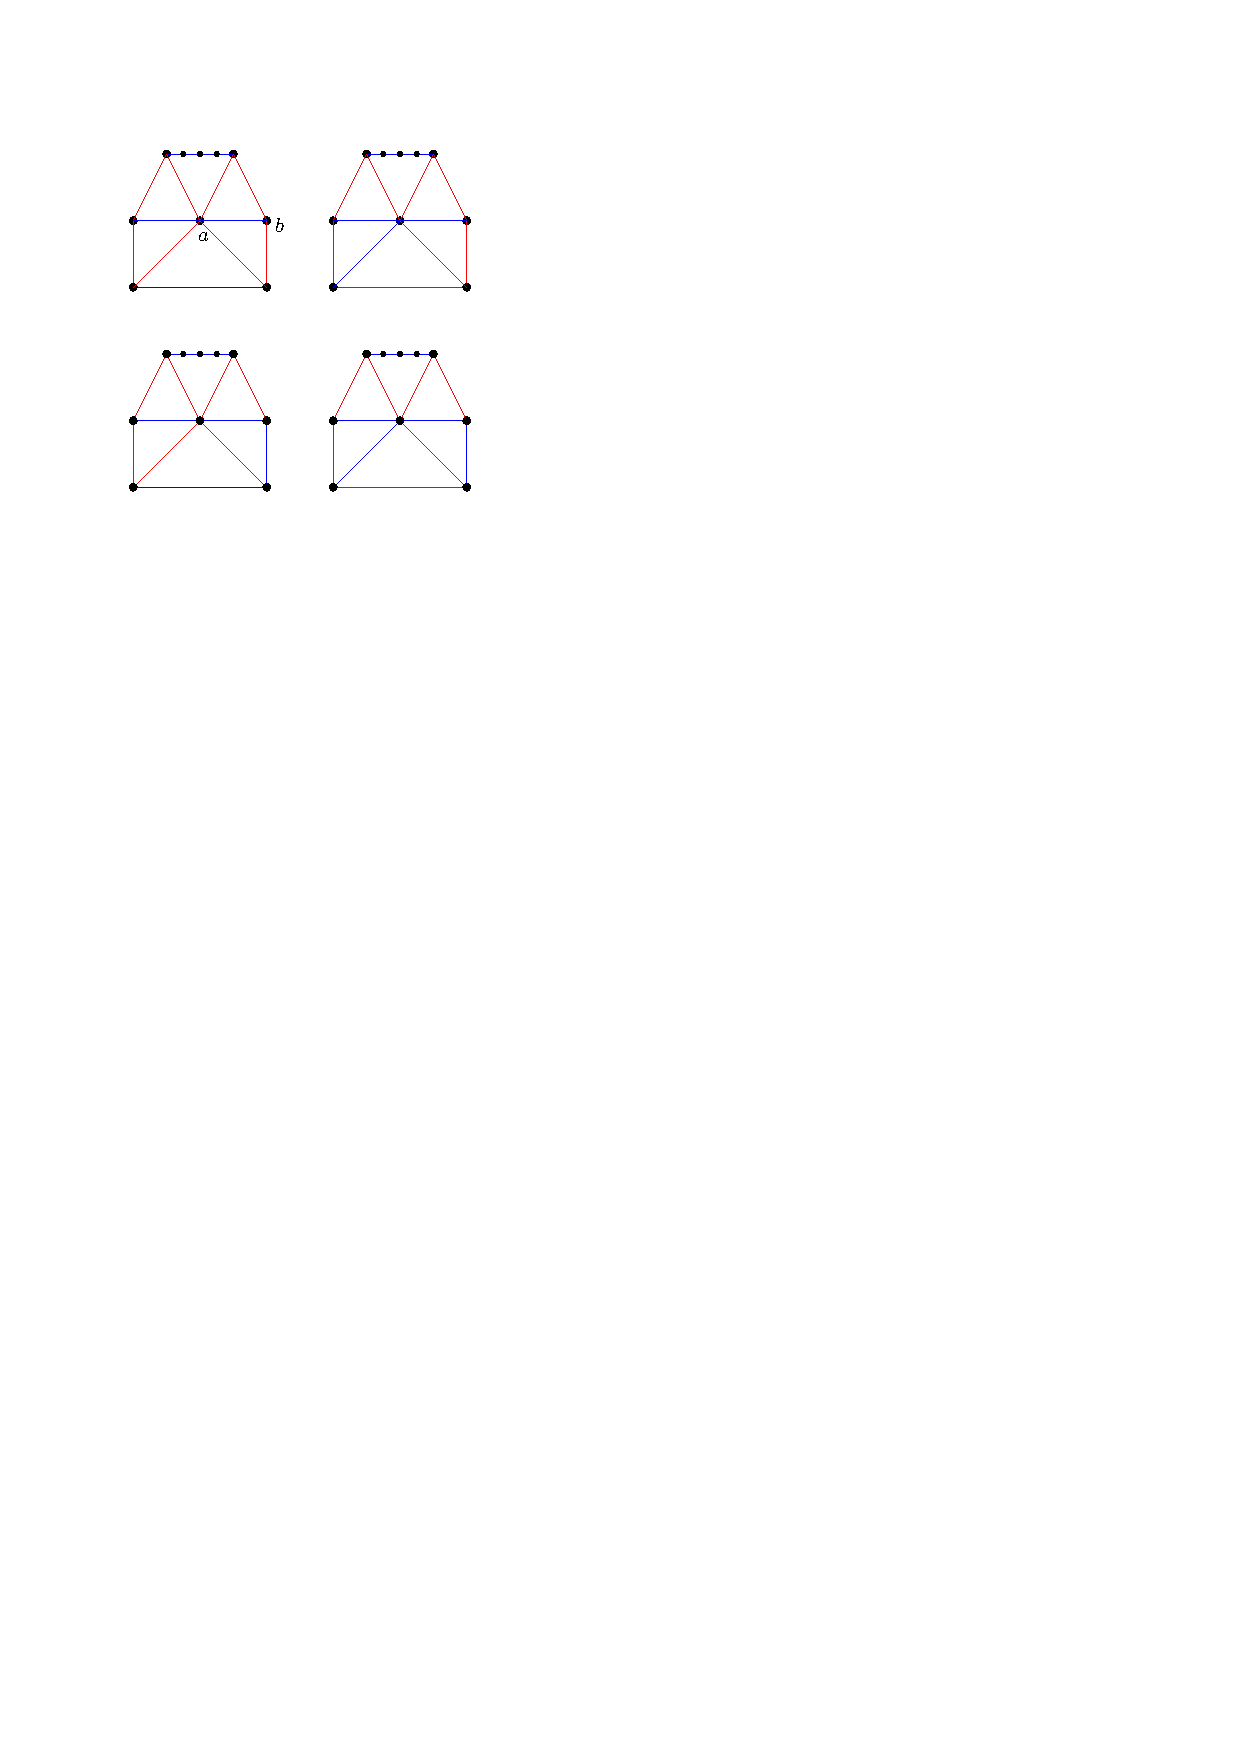
\includegraphics[scale=1]{chordReplace/img/options}
  \caption{}
  \label{fig:replace:options}
\end{figure}


Let us make a distinction between the cases when we have a single topfan and when we have multiple topfans. See Figure \ref{fig:replace:singleMultiTopFan}

\begin{figure}[h]
  \centering
  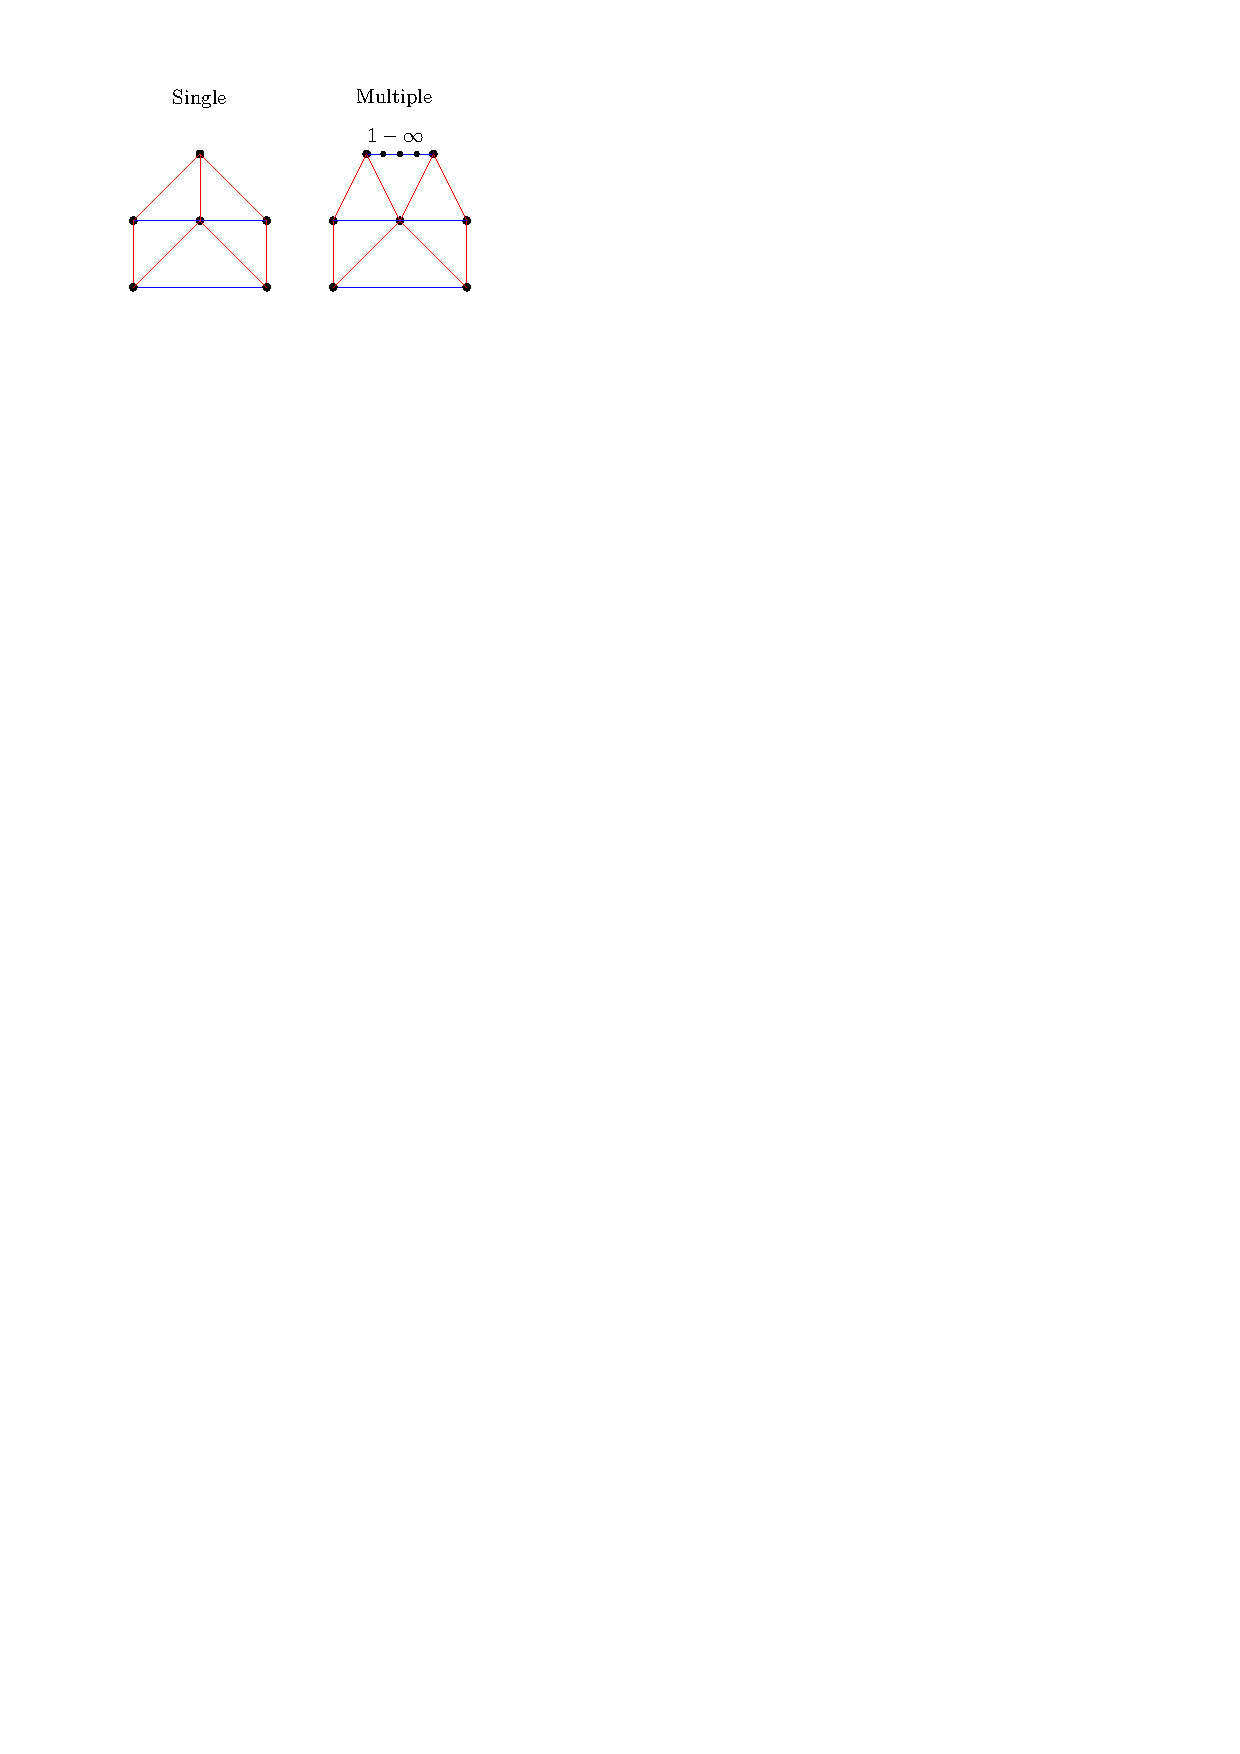
\includegraphics[scale=1]{chordReplace/img/singleMultiTopFan}
  \caption{}
  \label{fig:replace:singleMultiTopFan}
\end{figure}

\paragraph{Single topfan}
In case of the single topfan we can encouter two types of fanflips. Those of topfanse ending at the vertex $v$ or those of topfans extending past this vertex.

For the continuing topfans see Figure \ref{fig:replace:continueSingleTopFan} and for the stoping topfans see Figure \ref{fig:replace:stopSingleTopFan}


\begin{figure}
    \centering
    \begin{subfigure}[b]{0.45 \textwidth}
        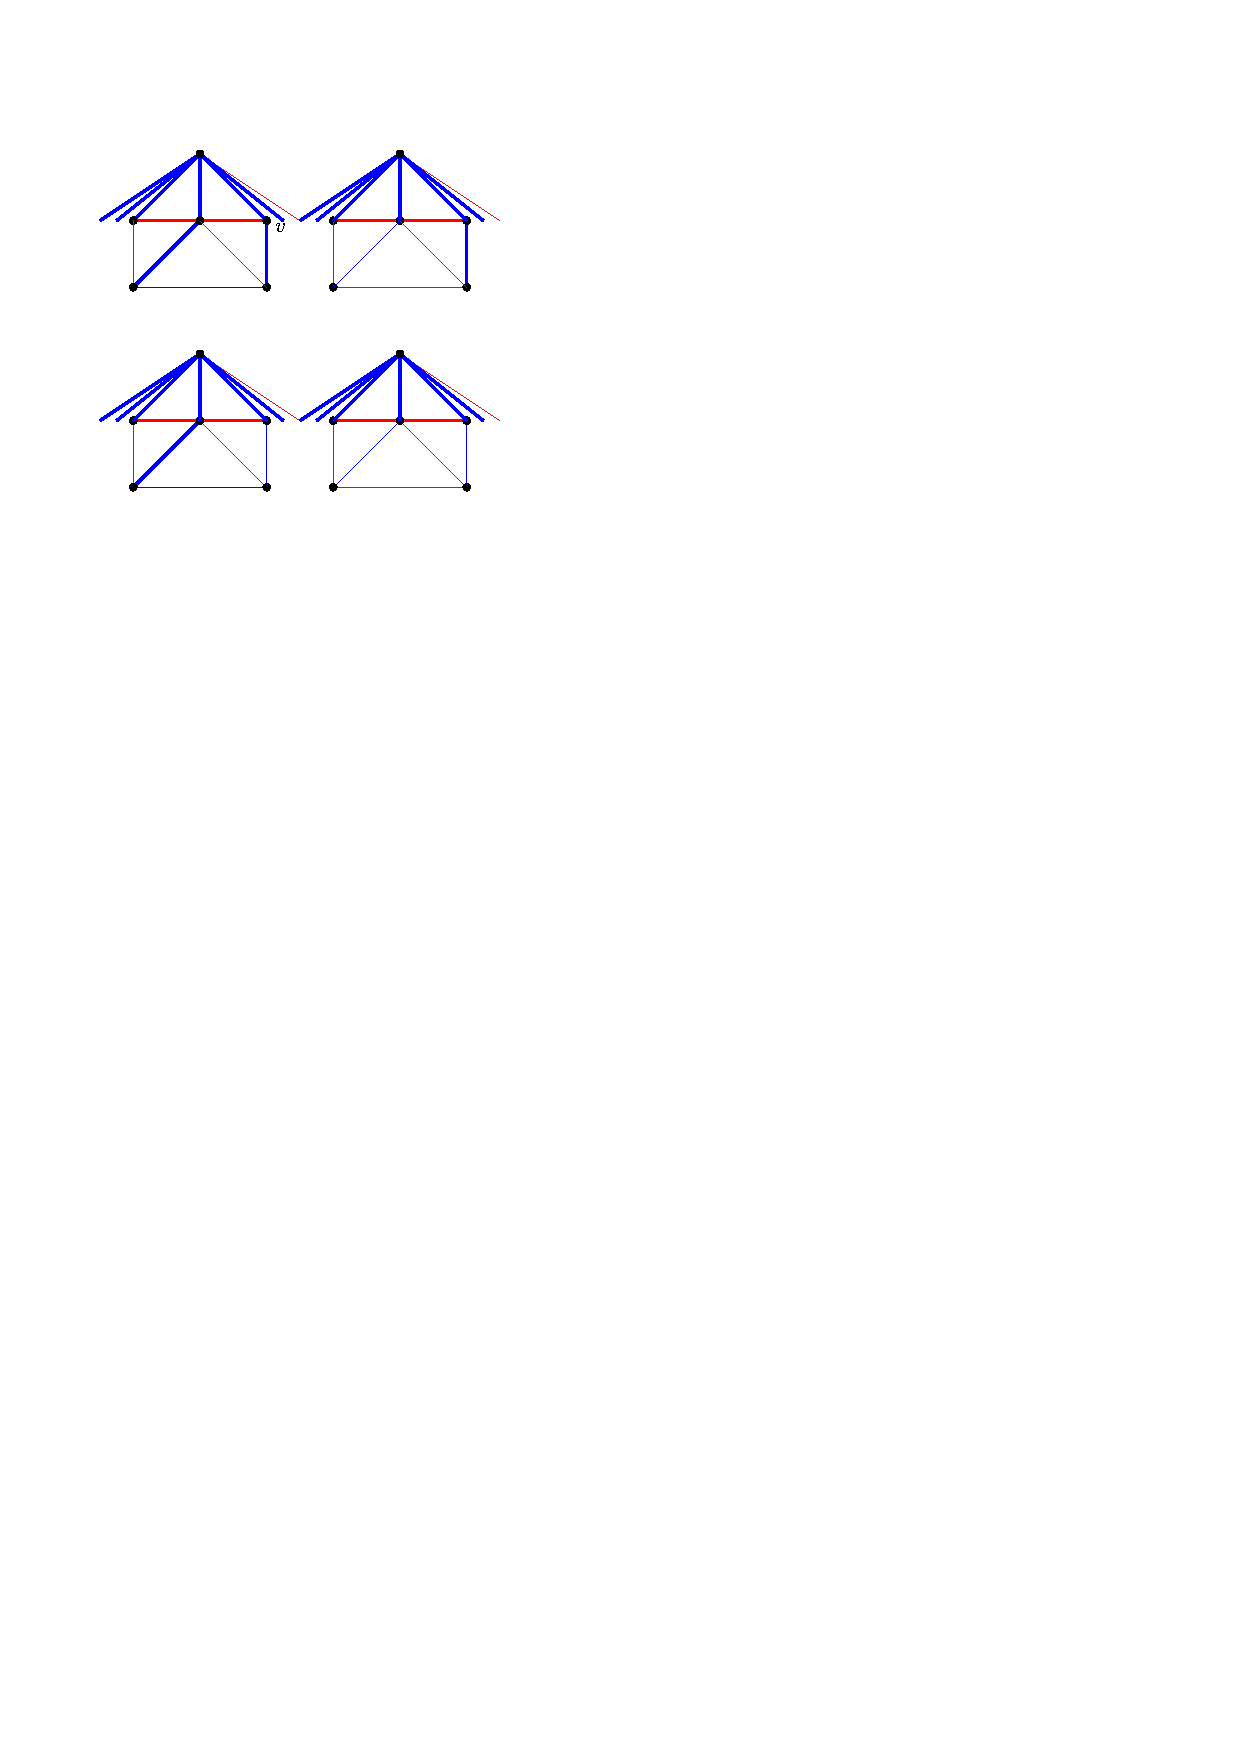
\includegraphics[width = \textwidth]{chordReplace/img/continueSingleTopFan}
        \caption{}
        \label{fig:replace:continueSingleTopFan}
    \end{subfigure}
    ~
    \begin{subfigure}[b]{0.45 \textwidth}
        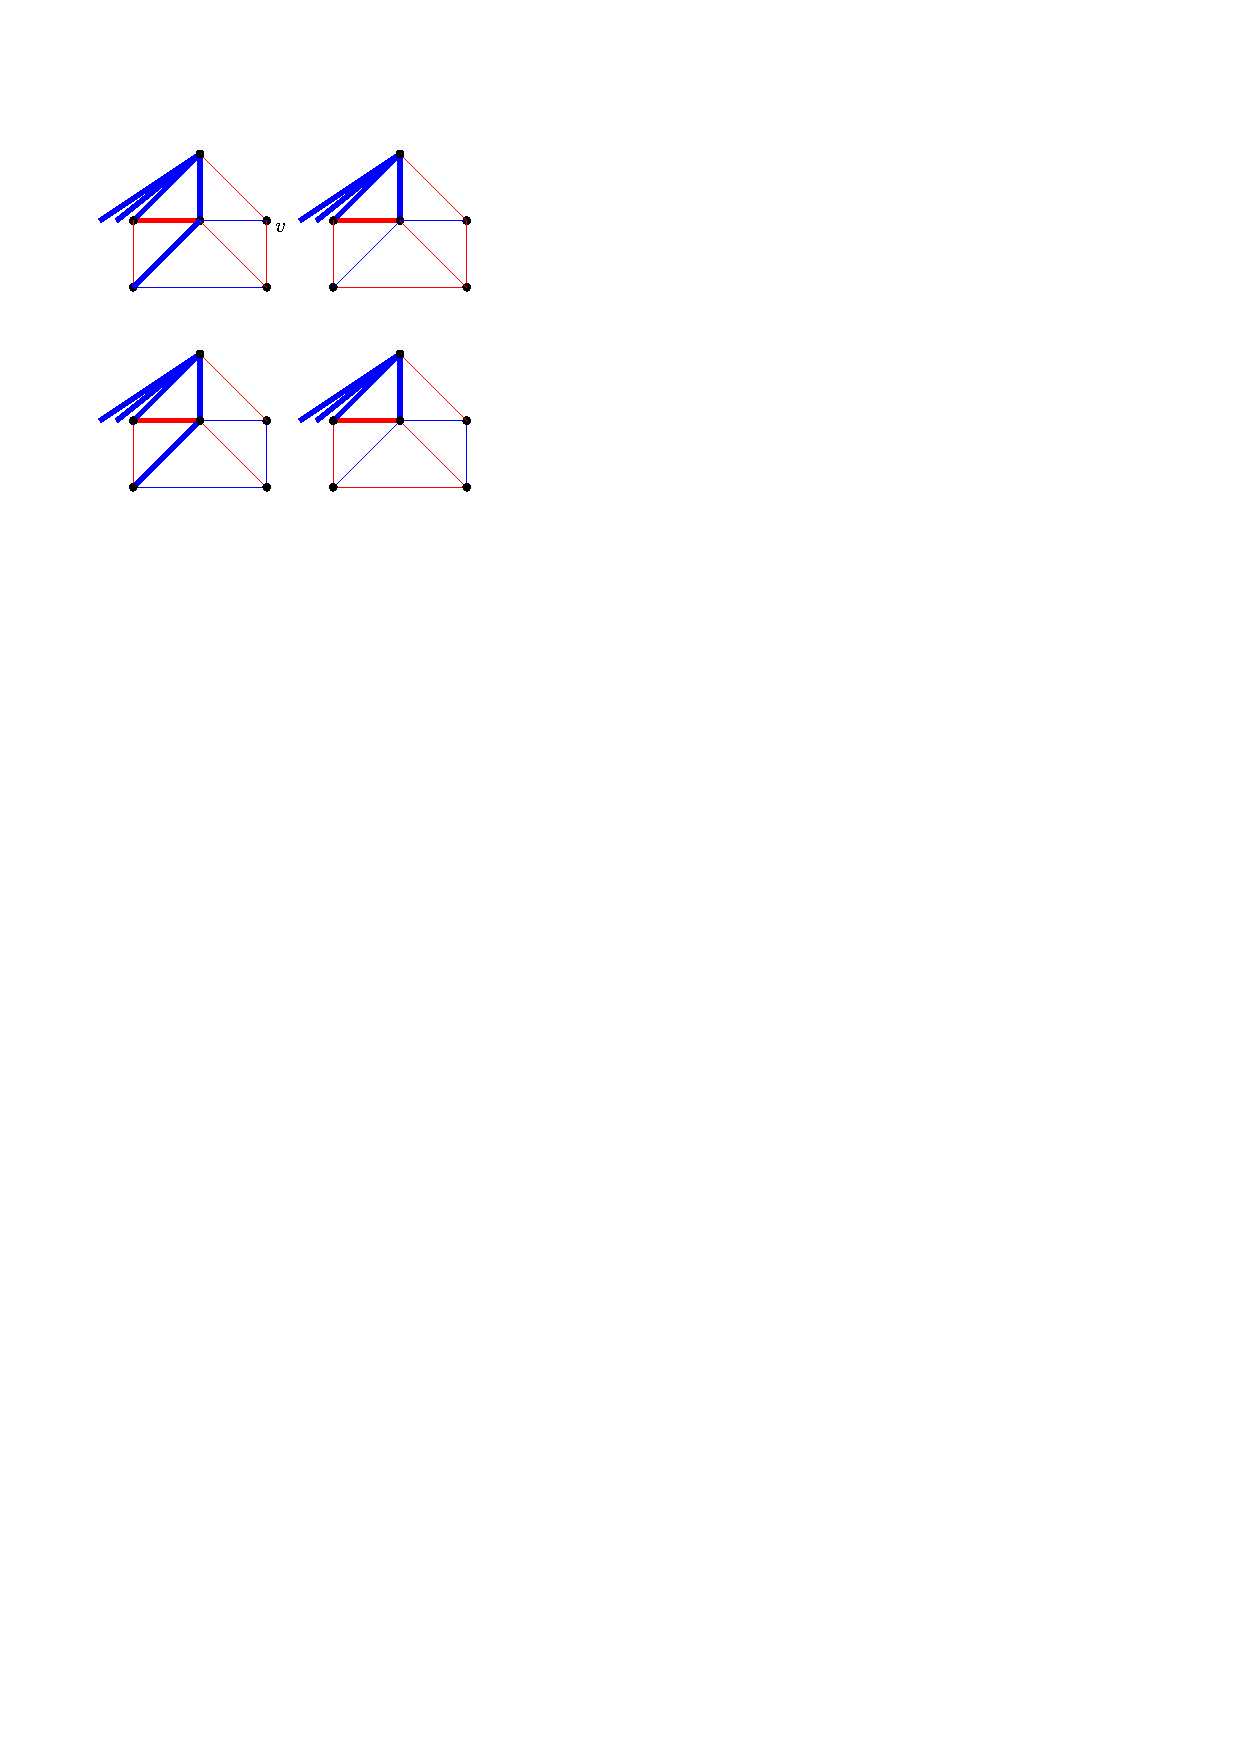
\includegraphics[width =\textwidth]{chordReplace/img/stopSingleTopFan}
        \caption{}
        \label{fig:replace:stopSingleTopFan}
    \end{subfigure}
    	\caption{}

\end{figure}

\paragraph{Mutiple topfans}
We are not influenced by a possible fanflip on the left topfan. Then the only thing we need to know is whether we flip the right topfan.

See Figure \ref{fig:replace:multiTopFan}.

\begin{figure}[h]
  \centering
  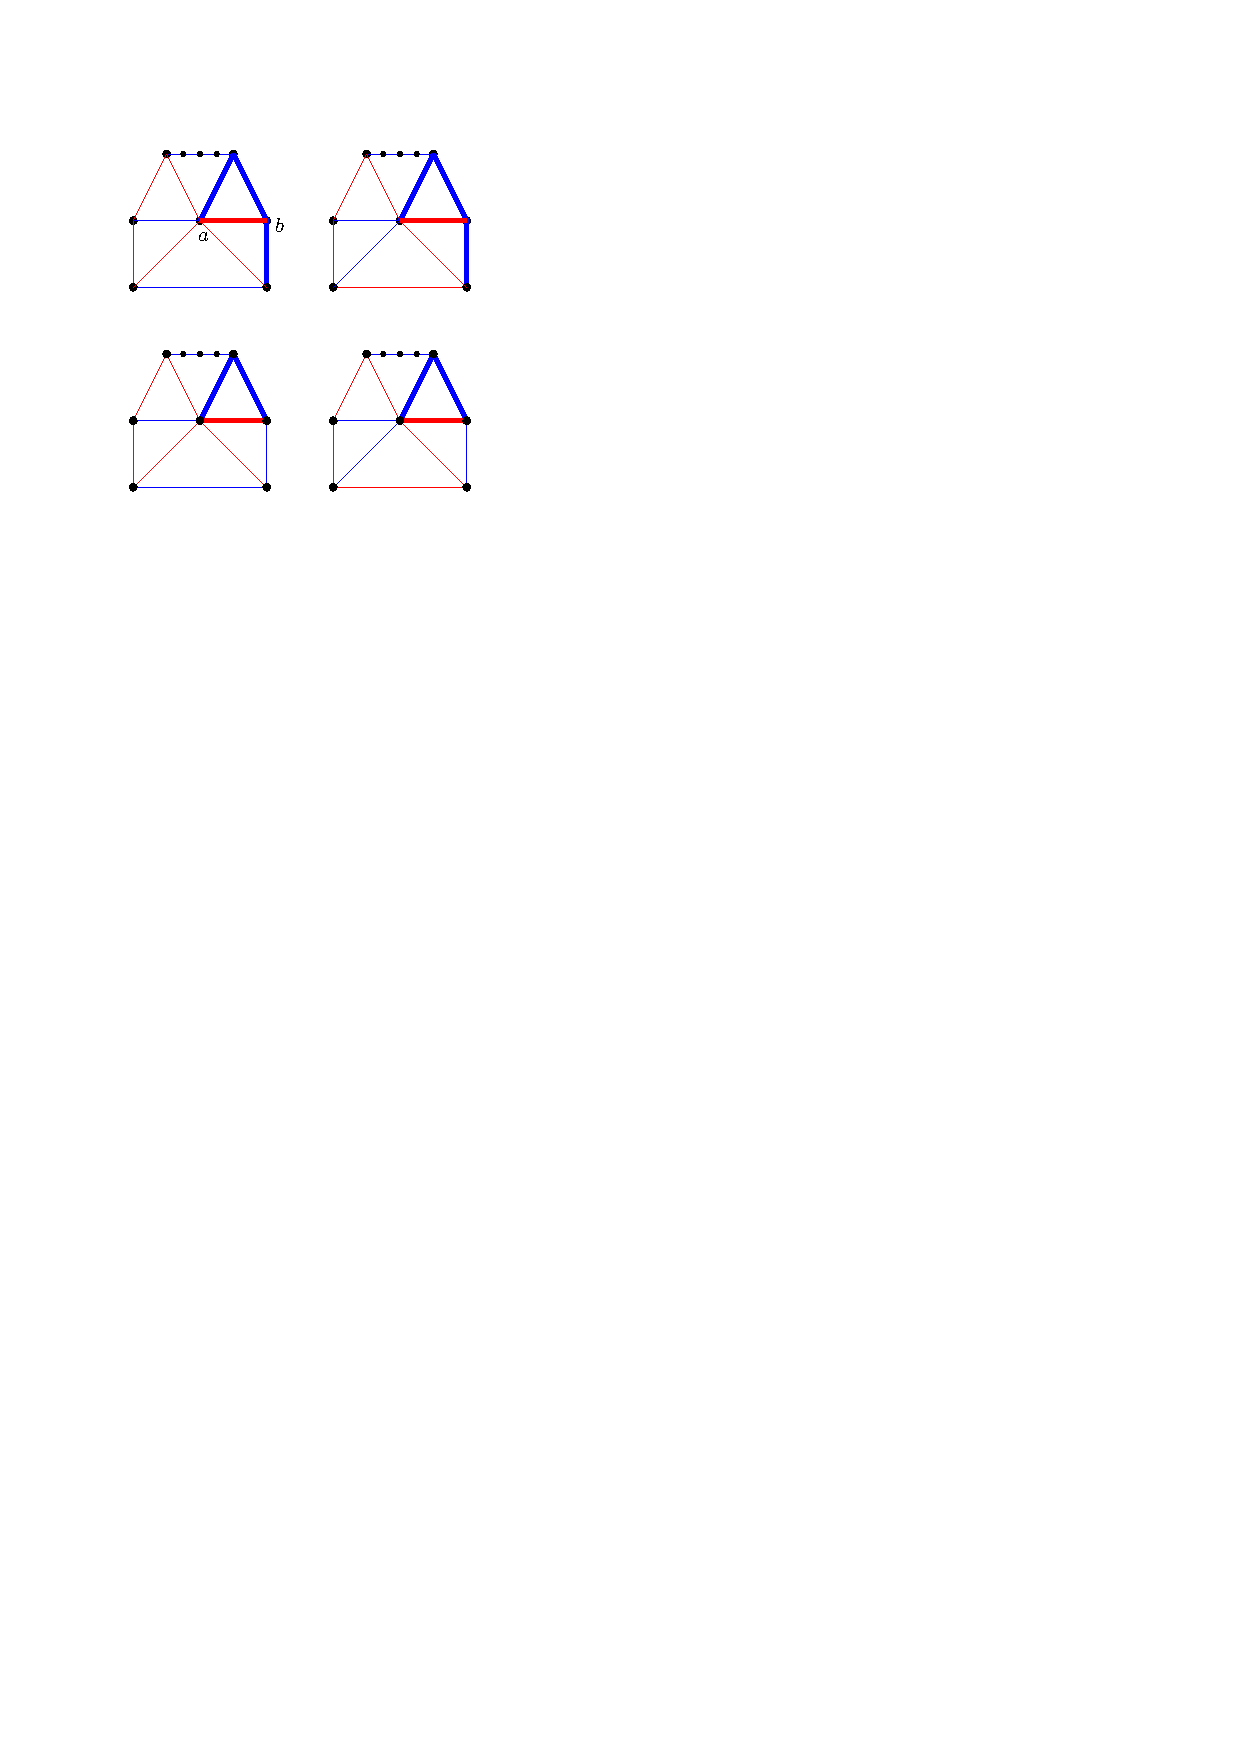
\includegraphics[scale=1]{chordReplace/img/multiTopFan}
  \caption{}
  \label{fig:replace:multiTopFan}
\end{figure}


\subsection{Replacing the chord}

We will show that for every possible state we can solve the original version of the subgraph while maintaining the edge coloring. We can see the unshrunk chord in Figure \ref{fig:replace:unshrunk}.

Note that the trivial chord corresponds to taking the minimum number along all 5 ranges.
\begin{figure}[h]
  \centering
  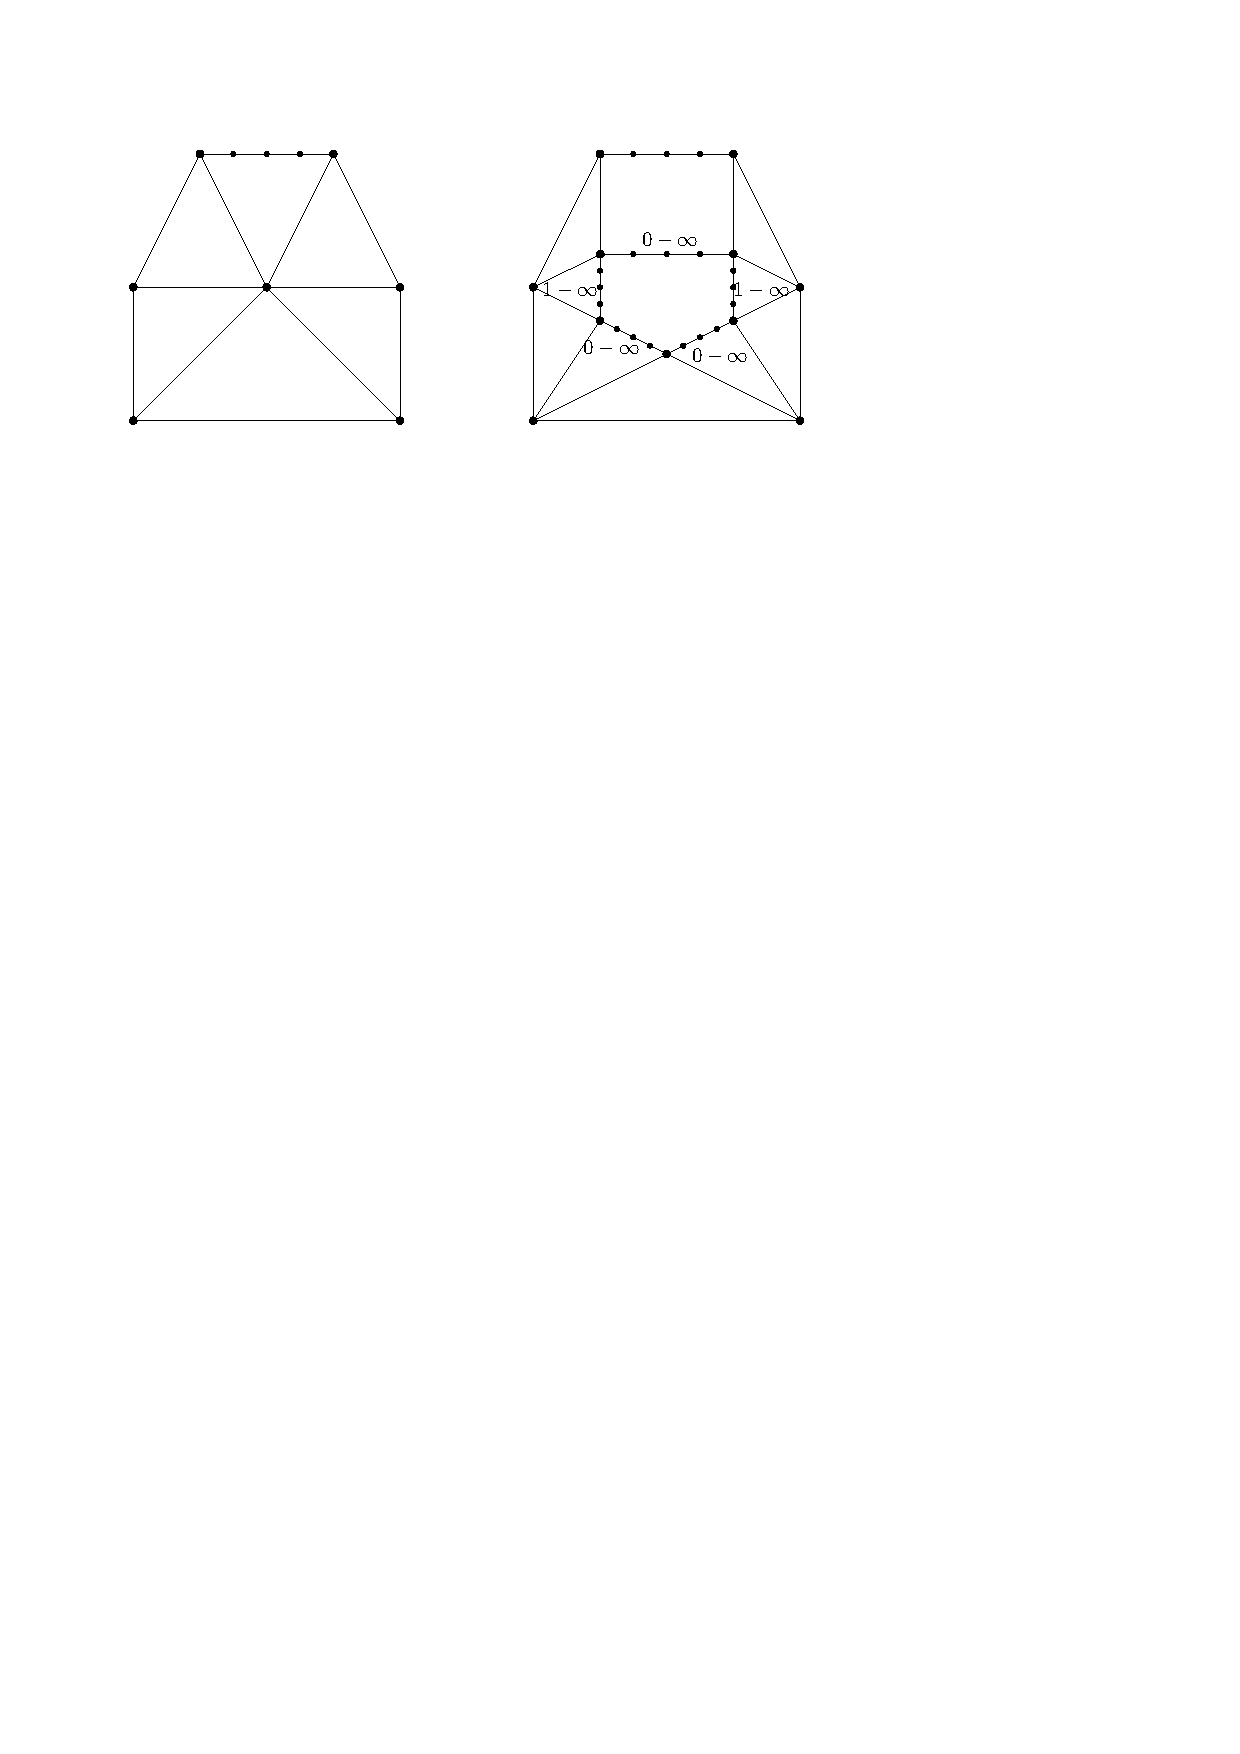
\includegraphics[scale=1]{chordReplace/img/unshrunk}
  \caption{Unshrink a chord}
  \label{fig:replace:unshrunk}
\end{figure}


 The coloring of the outside edges will have to be consistent. While we want the interior to remain without blue $Z$'s. We will want to have fans's whose coloring agrees with the original edges if this is possible. Except for maybe topfans if these would become large.



We will first show how we add poles and afterwards we debate whether this is useful.

\paragraph{Without fan flips}
See Figure \ref{fig:replace:polesNoFlip}. In all cases we enter with a valid sweeplinstate and without 4-cycles. (Except those with the $\pN$ vertex)

\begin{figure}[h]
  \centering
  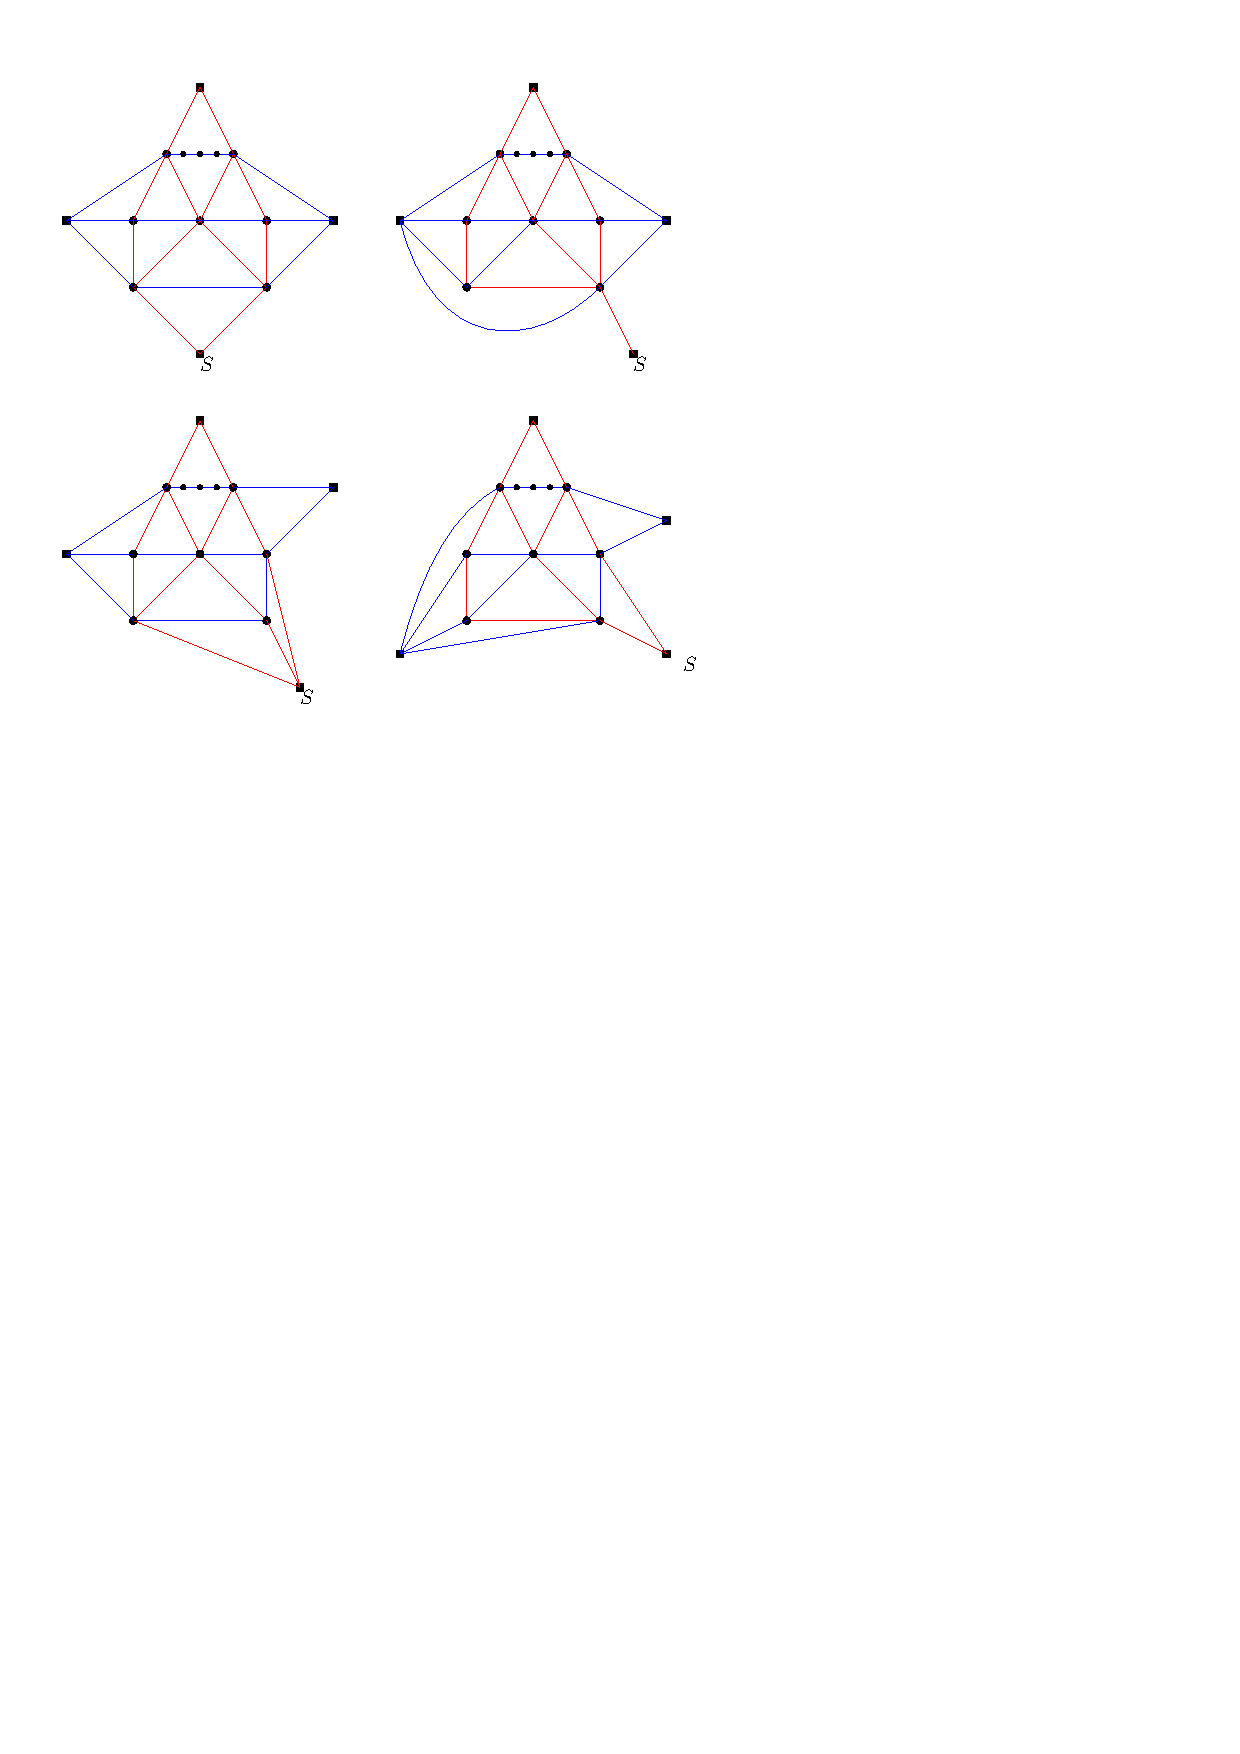
\includegraphics[scale=1]{chordReplace/img/polesNoFlip}
  \caption{}
  \label{fig:replace:polesNoFlip}
\end{figure}


\paragraph{With a single topfanflip}
Some resulting options of fan-flips and preflip states are the same so in total we end up with the following cases



\subsection{Warnings and remarks}

\fxwarning{For fan flips to work we must be careful around $4$-cycles}

For fan flips to work we require the absence of $4$-cycles. Unfortunately there can be


\fxwarning{When expending the chord we can get a large topfan. But those are large in this subgraph as well so hopefully fixed in the recursion?. More layers of recursion, but only maxdegree many. Or some other quatity expressing recurion depth. Maybe something with nested 5-cycles. If the same thing can't happen with multi topfans}
